\section{Træningsopgaver}


\subsection{Opgave 1}
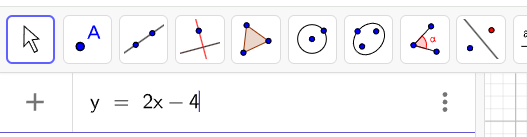
\includegraphics[scale=0.5]{img_1}

Find forskriften for linjen gennem 2 punkter som ses på billedet ovenfor: $y=ax+b$

For at finde forskriften for en ret linje skal vi først bestemme linjens hældning. Givet 2 punkter kan vi bestemme hældningen ved brug af følgende formel

\begin{frm-thm}{Hældningen af ret linje givet 2 punkter}\thlabel{a}

Givet punkterne $(x_1,y_1)$ og $(x_2,y_2)$ er hældningen, a, af den rette linje som går igennem disse punkter bestemt ved

\[a = \frac{y_2 - y_1}{x_2 - x_1}\]
\end{frm-thm}

Ud fra billedet kan vi aflæse punkternes koordinater og vi beregner hældningen til

\begin{align*}
a = \frac{y_2 - y_1}{x_2 - x_1} = \frac{5-2}{5-2} = \frac{3}{3} = 1
\end{align*}

Hældningen af den rette linje som går igennem punkterne på billedet er dermed $a=1$.

Når vi har beregnet hældningen mangler vi at beregne linjens skæring med y-aksen, b. For at beregne skæringen med y-aksen bruger vi følgende formel

\begin{frm-thm}{Den rette linjes skæring med y-aksen}\thlabel{b}

Givet et punkt $(x,y)$ på en ret linje og den rette linjes hældning a, kan den rette linjes skæring med y-aksen beregned ved

\[b = y-ax\]

\end{frm-thm}

Vi beregner den rette linjes skæring med y-aksen ved brug af punktet $(x_1,y_1) = (2,2)$, den rette linjes hældning $a = 1$ og formlen ovenfor

\begin{align*}
b=y-ax = 2-1\cdot 2 = 2 - 2 = 0
\end{align*}

Da vi både har den rette linjes hældning $a=1$ og dens skæring med y-aksen $b=0$ er forskriften for den rette linje som går gennem de 2 punkter på billeder givet ved

\begin{align*}
y = 1x+0 = x
\end{align*}

Vi kan altså både skrive $y = 1x + 0$ eller $y = x$.

\subsection{Opgave 2}
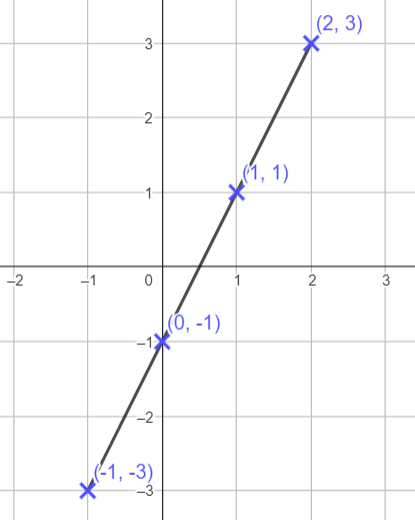
\includegraphics[scale=0.5]{img_2}

Givet ovenstående billede, aflæs hældningen, a og skærings med y-aksen, b.

For at aflæse hældningen, går vi 1 ud ad x-aksen, og bevæger os op eller ned ad y-aksen til vi støder på linjen. Det stykke vi har bevæget os op eller ned ad y-aksen før vi rammer linjen er hældningen. I dette tilfælde går vi altid 1 op ad y-aksen når vi går 1 hen ad x-aksen og hældnignen a er dermed $a=1$.
For at finde skæringen med y-aksen aflæser vi y-værdien i det punkt hvor linjen skærer y-aksen. I dette tilfælde skærer linjen i -1 dvs $b=-1$. Aflæsnignen af hældningen og skæringen med y-aksen kan ses på nedenstående billede.

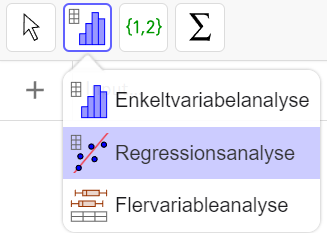
\includegraphics[scale=0.5]{img_3}

\subsection{Opgave 3}

Bestem skæringspunktet mellem de to linjer på nedenstående figur

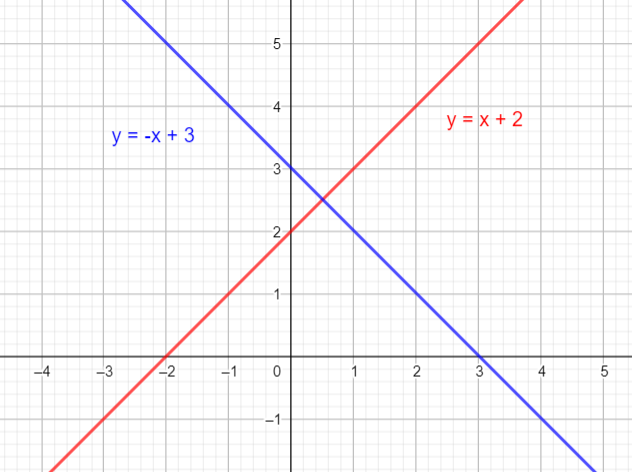
\includegraphics[scale=0.5]{img_4}

Vi bestemmer først skæringspunktet mellem de 2 linjer ved at aflæse på grafen. Kigger vi på figuren kan vi se at linjerne skærer hinanden i punktet $0.5, 2.5)$.

For at beregne skæringspunktet skal vi løse 2 ligninger med 2 ubekendte. For at løse 2 ligninger med 2 ubekendte gør vi følgende

Først sætter vi de 2 ligninger lig med hinanden

Derefter isolerer vi x for at finden x-værdien

Til sidst indsætter vi den fundne x-værdi i en af de 2 ligninger for at beregne y-værdien.

De fundende x og y værdier er dermed skæringsunktet $(x,y)$ mellem de 2 linjer.

\begin{align*}
x+2 &= -x+3\\
\Updownarrow \hspace*{16mm}&\\
x + 2 - 2 &= -x + 3 - 2\\
\Updownarrow \hspace*{16mm}&\\
x &= -x + 1\\
\Updownarrow \hspace*{16mm}&\\
x + x &= -x + 1 + x\\
\Updownarrow \hspace*{16mm}&\\
2x &= 1\\
\Updownarrow \hspace*{16mm}&\\
\frac{2x}{2} &= \frac{1}{2}\\
\Updownarrow \hspace*{16mm}&\\
x &= \frac{1}{2}
\end{align*}

Skæringspunktets x-kordinat er dermed $x = 0.5$. Vi finder y-koordinatet til skæringspunktet ved at indsætte x-værdien på x's plads i en af de 2 ligninger.

\begin{align*}
y = x + 2 =  0.5 + 2 = 2.5
\end{align*}

Skæringspunktet mellem de 2 linjer er dermed $(0.5, 2.5)$, som var det vi aflæste på grafen.


For at tjekke om vi har aflæst og bergnet skæringspunktet korrekt, kan vi plotte de 2 ligninger i geogebra og bruge skæringsværktøjet som ses på billedet nedenfor

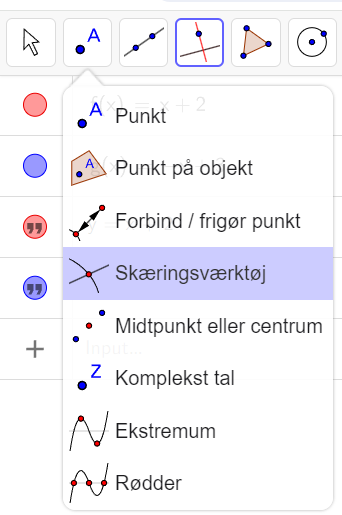
\includegraphics[scale=0.5]{img_5}

Herefter klikker man på de 2 linjer og skæringspunktet kommer frem som kan ses på nedenstående billede

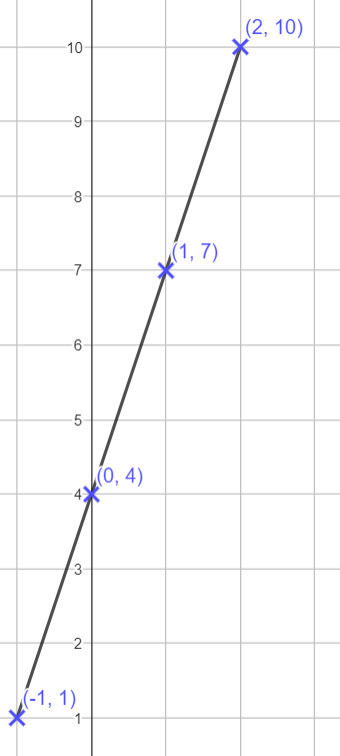
\includegraphics[scale=0.5]{img_6}

Som vi kan se på billedet giver skæringsværktøjet i geogebra det samme resultat som vi gar beregnet.

\subsection{Opgave 4}

I denne opgave skal vi kigge på hvordan man laver regresionsanalyse i geogebra givet en række punkter. Vi er givet følgende punkter

\begin{tabular}{c|c}
x & y\\
\hline
1 & 0.50\\
2 & 1.00\\
3 & 1.45\\
4 & 2.03
\end{tabular}

I geogebra vælger man regneark som kan ses på endenstående billede 

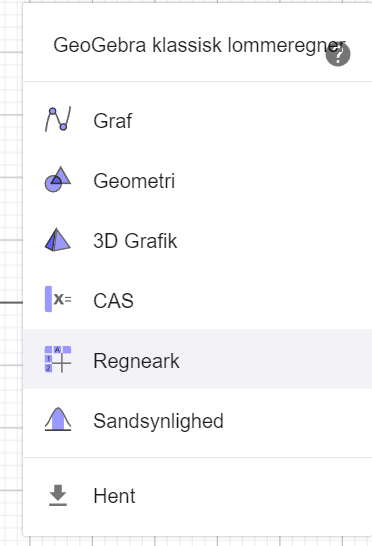
\includegraphics[scale=0.5]{img_7}

Derefter skriver man punkterne ind, x værdierne i den første kolonne, og y værdierne i den anden kolonne. Dette kan ses på nedenstående billede

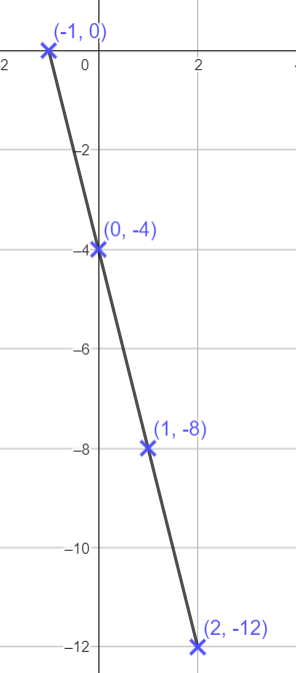
\includegraphics[scale=0.5]{img_8}

Vi markerer alle punkterne i regnearket og vælger regressionsanalysen.

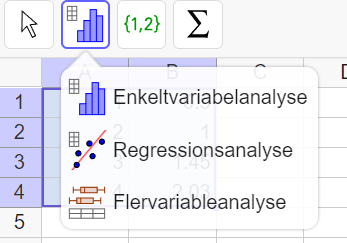
\includegraphics[scale=0.5]{img_9}

Nu ser vi et vindue med vores punkter indtegnet.

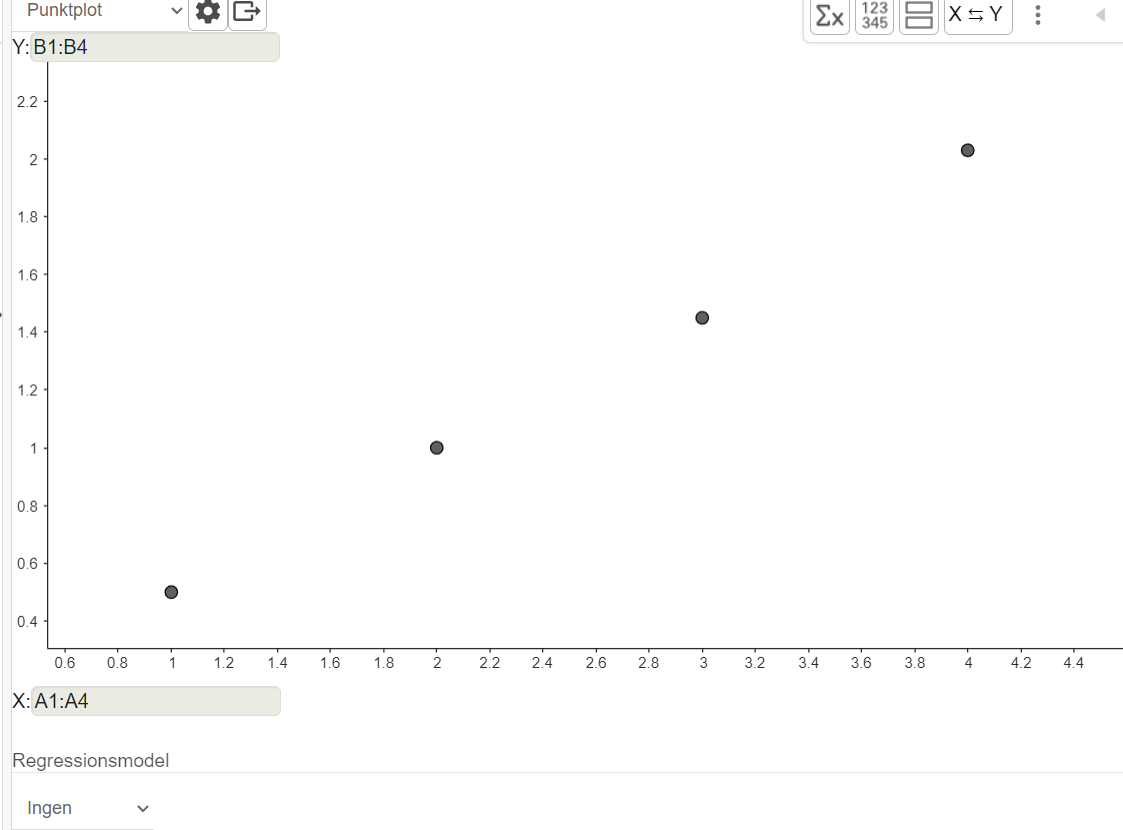
\includegraphics[scale=0.5]{img_10}

Nu klikker vi på boksen hvor der står regressionsmodel og vælger lineær.

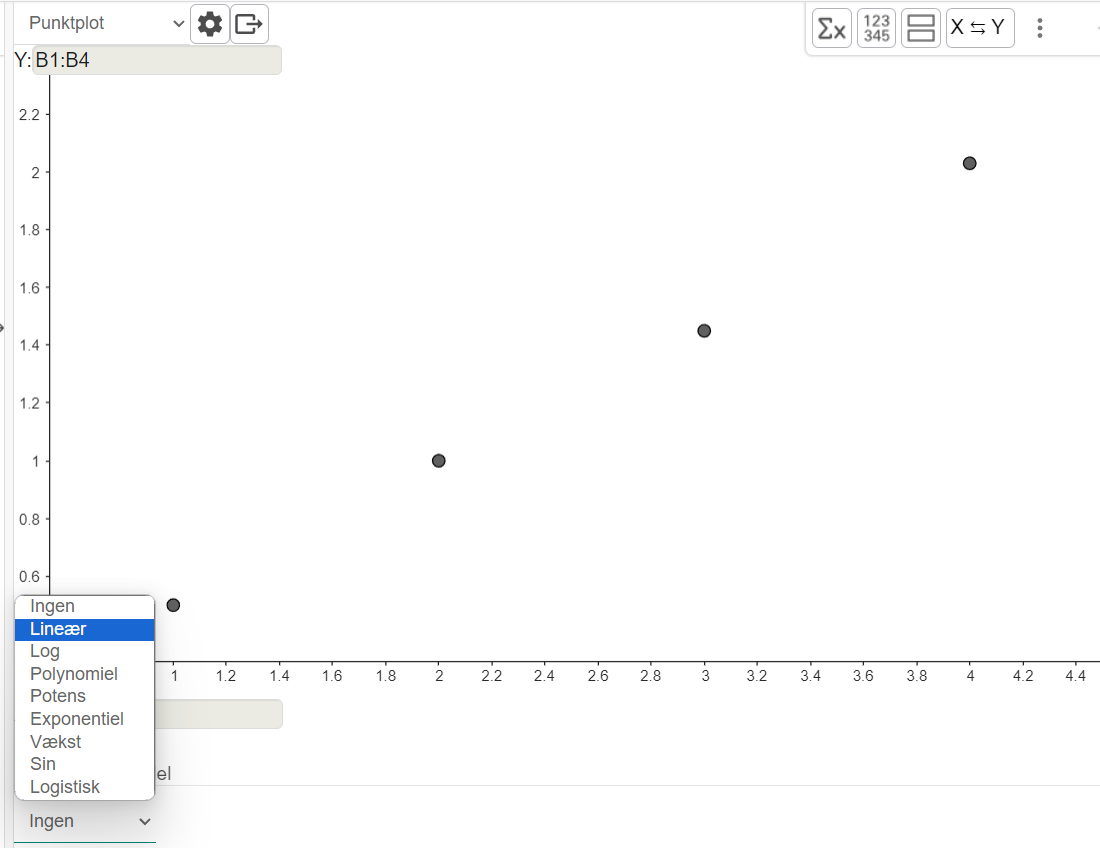
\includegraphics[scale=0.5]{img_11}

Geogebra laver nu en ret linje som rammer de 4 punkter bedst muligt som kan ses nedenfor.

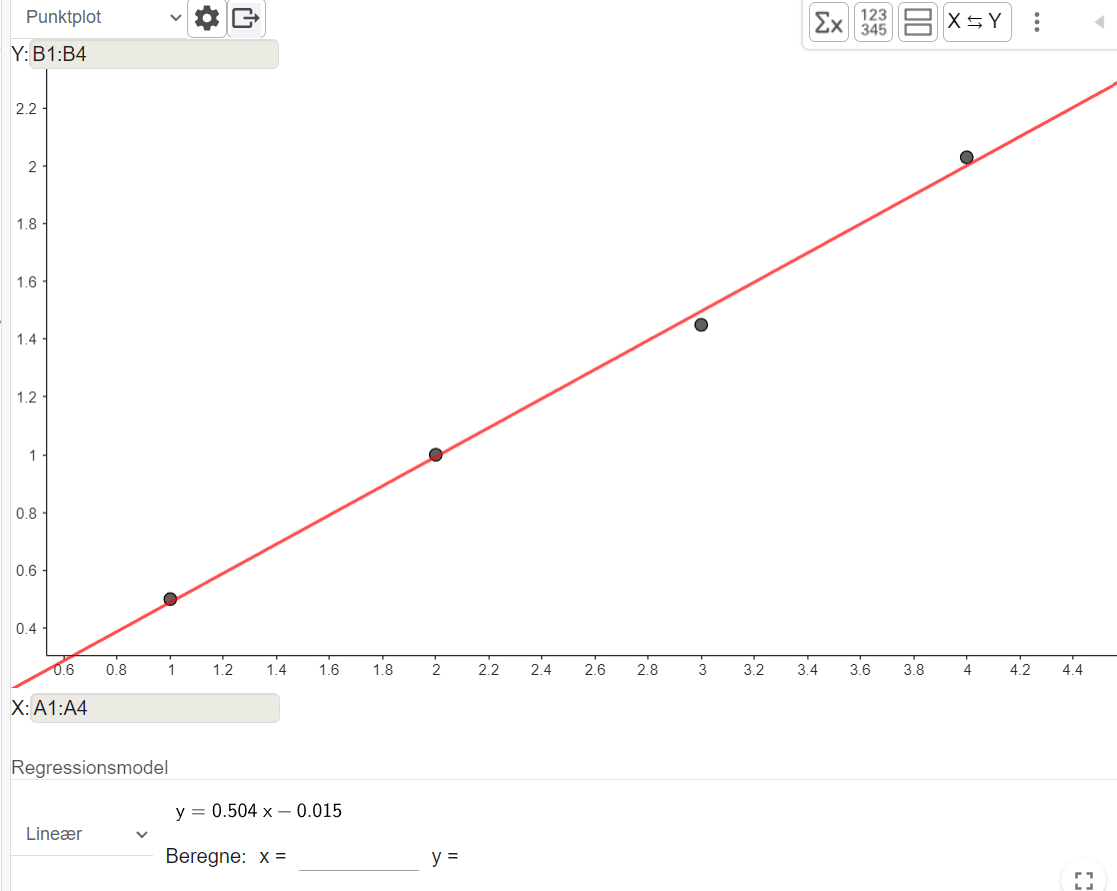
\includegraphics[scale=0.5]{img_12}



